\chapter{Conceitos básicos de aprendizagem de máquina}
\label{cap:conceitos-basicos-aprendizagem-maquina}

\framebox[\textwidth]{
	\hspace{1em}
	\vbox{
		\textbf{Leitura obrigatória:}
		\begin{itemize}
			\item \cite{FaceliEtAl2011} -- Cap. 1 (Introdução).
			\item \cite{MullerAndGuido2017} -- Cap. 1 (Introduction).
		\end{itemize}
		
		\textbf{Leitura complementar:}
		\begin{itemize}
			\item \cite{Mitchell1997} -- Cap. 1 (Introduction).
			\item \cite{FaceliEtAl2011} -- Cap. 2 (Análise de Dados).
		\end{itemize}
	}
}

\section{O que é aprendizagem de máquina?}

A ideia fundamental da aprendizagem de máquina é fazer com que o agente melhore o seu desempenho na execução de alguma tarefa. Muitas vezes é impossível programar um agente que execute uma determinada tarefa com qualidade. Por exemplo, implementar um agente capaz de reconhecer pessoas pela sua face e sua voz poderia exigir que todas as situações possíveis sejam levadas em conta durante o projeto. Uma pessoa pode ter sua voz alterada por conta de um resfriado, ou por estar ofegante após realizar alguma atividade física. A face também pode ser alterada pelo crescimento da barba ou uso de um óculos. Agentes dessa natureza aprendem quais os padrões que devem ser reconhecidos para identificação e usam experiências anteriores para identificarem novas imagens.

Um segundo exemplo consiste no diagnóstico de doenças. Não existe um conjunto de regras predefinidas que mapeiem sintomas a doenças. Geralmente, o médico utiliza sua formação e experiência para realizar esta identificação. Um agente que execute esta tarefa deve aprender a diagnosticar com base em dados anteriores, de tal forma que possa fazê-lo com qualidade.

Em outros casos, o nível de processamento necessário para executar uma tarefa é muito alto, ou a quantidade de dados a serem analisados é muito grande. Por exemplo, dado um banco de dados com milhões de registros de vendas de uma loja, encontrar o produto mais vendido ou o vendedor com maior valor de comissão são tarefas simples de serem implementadas. No entanto, considere as tarefas de \textit{identificar conjuntos de produtos que são frequentemente vendidos juntos}, ou \textit{recomendar novos produtos a clientes que costumam comprar produtos semelhantes}. Estas tarefas são difíceis ou até mesmo impossíveis a seres humanos. Escrever um programa para fazê-lo também não é simples. Nestes casos, os algoritmos de aprendizagem de máquina fazem com que o agente aprenda a realizar estas tarefas.

Logo, a \textbf{aprendizagem de máquina} é um ramo da inteligência artificial que busca resolver problemas reais que um software simples não é capaz. Neste sentido, estes algoritmos resolvem os problemas criando por si próprios uma hipótese ou função com base em experiências anteriores. A este processo de indução de uma hipótese (ou função) a partir da experiência passada damos o nome de aprendizagem de máquina. Alguns exemplos de aplicações bem sucedidas de técnicas de aprendizagem de máquina incluem:

\begin{itemize}
	\item Reconhecimento de fala.
	\item Detecção de fraudes no uso de cartões de crédito.
	\item Direção autônoma de veículos em rodovias.
	\item Programas que jogam gamão e xadrez.
	\item Diagnóstico de câncer.
\end{itemize}


\section{Tarefas de aprendizagem}

Para detalhar o processo de indução de hipóteses, vamos considerar uma base de dados referentes aos pacientes de um hospital. Cada dado (também chamado de objeto, exemplo, padrão ou registro) corresponde a um paciente e é composto por uma tupla com suas características ou atributos (também chamados de campos ou variáveis). Por exemplo, os atributos podem ser o nome, idade, sexo, peso, sintomas, etc. Algumas tarefas de aprendizado definem um atributo como atributo de saída (também chamado atributo alvo ou atributo meta), cujos valores podem ser estimados em função dos demais, neste caso chamados de atributos de entrada (ou ainda atributos previsores). Em outras palavras, estas técnicas de aprendizagem de máquina tem por objetivo aprender uma hipótese que relacione os atributos de entrada com o atributo de saída, de tal forma que o valor do atributo de saída de novos pacientes possa ser estimado a partir dos valores dos seus atributos de entrada.

Quando o atributo alvo que se deseja determinar é um elemento de um conjunto discreto de valores, temos uma tarefa de \textbf{classificação}. Por exemplo, podemos determinar se um paciente está doente com base na sua temperatura, pressão arterial e se o mesmo está com dor de cabeça. O atributo alvo consiste no estado do paciente e pode assumir os valores (as classes) \textit{doente} ou \textit{saudável}. Quando o atributo alvo é uma variável contínua, temos um problema de \textbf{regressão}. Por exemplo, podemos determinar a gravidade da doença de acordo com os sintomas observados, podendo assumir um valor no intervalo $[0, 1]$.

Outras tarefas de aprendizagem não se baseiam em um atributo alvo a ser determinado, mas na extração de outras informações. A tarefa mais comum é o \textbf{agrupamento}, que consiste em dividir os objetos em grupos de acordo com os seus atributos. Por exemplo, o agrupamento pode ser aplicado para identificar os pacientes sujeitos a contrair uma virose, com base nos seus demais atributos. Outra tarefa que não se baseia em um atributo alvo é a \textbf{associação}, que busca identificar relações existentes entre diferentes grupos de atributos. Por exemplo, um algoritmo de associação poderia identificar que os pacientes que apresentam manchas na pele possuem um baixo nível de glóbulos brancos no sangue. O usuário pode utilizar este tipo de informação para gerar novos conhecimentos ou tomar decisões.

\section{Classificação dos algoritmos}

Os algoritmos de aprendizagem de máquina são classificados de acordo com o paradigma de aprendizado no qual se aplicam. Existem três principais tipos: aprendizado supervisionado, aprendizado não supervisionado e aprendizado por reforço.

O \textbf{aprendizado supervisionado} agrega os métodos que buscam induzir uma hipótese que relacione os atributos de entrada com um atributo alvo. Por conta disso, estes métodos são também chamados de \textbf{métodos preditivos}. Como visto na seção anterior, dois exemplos deste tipo de abordagem são a classificação e a regressão. O aprendizado é chamado supervisionado pois os métodos se baseiam em um conjunto de dados rotulados, onde já se conhece o valor do atributo alvo. Isto é, este conjunto de dados atua como um ``supervisor externo'', que conduz os algoritmos para a indução da hipótese.

O \textbf{aprendizado não supervisionado} agrega os métodos que exploram e descrevem um conjunto de dados e, portanto, não fazem uso de um atributo alvo. Por isso, estes métodos são chamados de \textbf{métodos descritivos}. Como visto na seção anterior, as principais tarefas do aprendizado não supervisionado são o agrupamento e a associação.

Finalmente, o \textbf{aprendizado por reforço} considera um agente que deve executar uma tarefa de qualquer natureza. O ambiente é responsável por oferecer uma recompensa conforme a ação tomada pelo agente. Caso a ação seja desejada, a recompensa é positiva, caso contrário, a recompensa é negativa. Através da experiência em várias tentativas, o agente ajusta seu comportamento conforme a recompensa recebida do sistema e, com isso, aprende o comportamento desejado. Um exemplo consiste em um robô que deve aprender um caminho entre dois pontos de um prédio.

\begin{figure}[h]
	\centering
	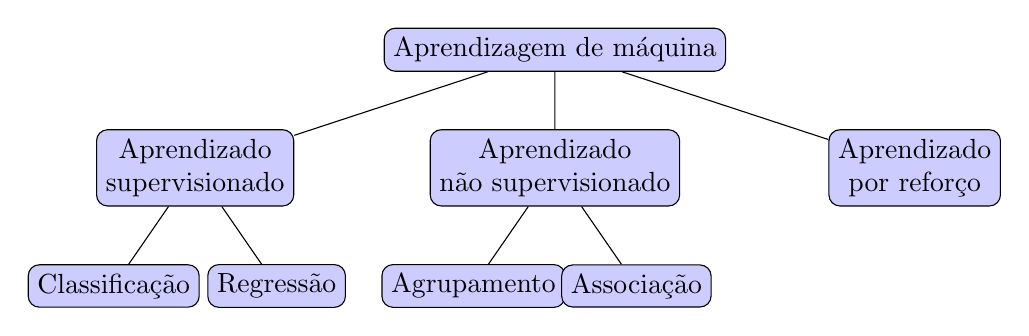
\begin{tikzpicture}[sibling distance=13em,every node/.style = {shape=rectangle, rounded corners,draw,align=center,fill=blue!20}]]
		
		\node {Aprendizagem de máquina}
		child { node {Aprendizado\\supervisionado}
			child{ node at (1.25,0) {Classificação}}
			child{ node at (-1.25,0) {Regressão}}
		}
		child { node {Aprendizado\\não supervisionado}
			child{ node at (1.25,0) {Agrupamento}}
			child{ node at (-1.25,0) {Associação}}	
		}
		child { node {Aprendizado\\por reforço} };
			
	\end{tikzpicture}

	\caption{Taxonomia dos principais métodos e tarefas de aprendizagem de máquina}
	\label{fig:taxonomia-aprendizagem-maquina}
\end{figure}

A Figura~\ref{fig:taxonomia-aprendizagem-maquina} apresenta uma taxonomia com base nas informações apresentadas. A aprendizagem de máquina se divide em aprendizado supervisionado, aprendizado não supervisionado e aprendizado por reforço. O aprendizado supervisionado é composto pelas tarefas de classificação e regressão, enquanto o aprendizado não supervisionado é composto pelas tarefas de agrupamento e associação. Este material apresenta os métodos de aprendizagem de máquina seguindo esta organização.

\section{Overfitting e underfitting}

Um importante conceito inerente a qualquer tarefa de aprendizagem é a generalização da hipótese induzida. Dizemos que uma hipótese possui boa generalização quando ela funciona adequadamente para novos objetos. No entanto, alguns problemas podem fazer com que os algoritmos resultem em hipóteses com baixa generalização. O principal deles é chamado de \textit{overfitting} (ou sobreajuste), que acontece quando a hipótese está especializada nos dados de treinamento, e não consegue predizer com qualidade para novos dados. Em outras palavras, quando o modelo se ajusta demasiado aos dados existentes, ele torna-se complexo e não generaliza para novos dados.

Por outro lado, quando o modelo é simplificado demais, ele não possui boa performance, nem sobre o conjunto de dados existentes, nem sobre novos dados. Esta característica é chamada de \textit{underfitting} (ou subajuste). O ideal, portanto, consiste em encontrar um modelo que possua boa performance nos dados existentes e ao mesmo tempo seja simples o suficiente para uma boa generalização a novos dados.

\begin{figure}[h]
	\centering
	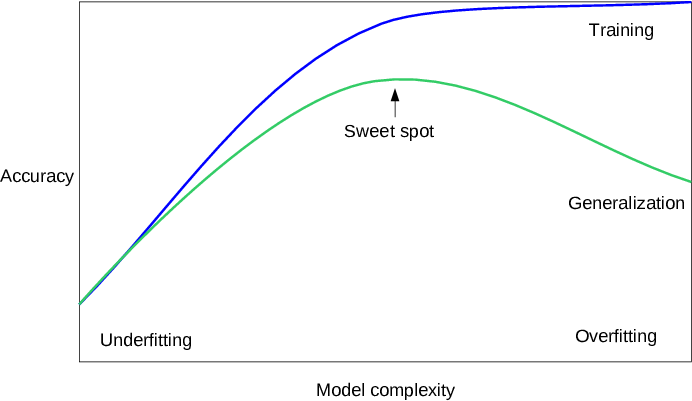
\includegraphics[width=0.7\textwidth]{img/overfitting-underfitting}
	\caption{Trade-off entre complexidade do modelo e generalização}
	\label{fig:overfitting-underfitting}
\end{figure}

A Figura~\ref{fig:overfitting-underfitting} ilustra estes problemas. Quando o modelo se ajusta demais aos dados (curva em azul), a complexidade aumenta e a generalização diminui. O ponto ótimo (representado pelo \textit{sweet pot}) possui uma complexidade intermediária, capaz de responder com qualidade aos dados existentes e novos.

\section{Repositório de dados}

No projeto e desenvolvimento de métodos de aprendizagem de máquina, é comum o uso de conjuntos de dados comuns e disponíveis à comunidade científica. Isso facilita a execução de experimentos, pois o projetista não precisa se preocupar em preparar diferentes conjuntos de dados, bem como permite a comparação de distintas técnicas em um número maior de bases de dados.O repositório mais conhecido é o UCI, que pode ser acessado no endereço \url{http://archive.ics.uci.edu/ml}. Este repositório possui 383 conjuntos de dados que podem ser utilizados para aplicação de diferentes métodos de aprendizagem de máquina. Para cada conjunto de dados, são apresentadas suas informações básicas (número de instâncias, números de atributos, tarefa de aprendizagem associada, etc.), uma descrição sobre a origem dos dados e artigos científicos relacionados.

O conjunto de dados das espécies de íris, por exemplo, pode ser consultado em \url{http://archive.ics.uci.edu/ml/datasets/Iris}. Ele possui 150 instâncias, cada uma com 4 atributos e a tarefa de aprendizagem é a classificação. Com base nos 4 atributos de entrada, a tarefa consiste em determinar uma entre as três classes possíveis (\textit{íris setosa}, \textit{íris versicolor} e \textit{íris virgínica}). Os dados são disponibilizados em um arquivo com extensão \texttt{.data} e possuem uma estrutura simples que facilita sua leitura. O arquivo \texttt{iris.data} apresenta o valor de cada atributo separado por vírgula, com a classe sendo apresentada por último (Figura~\ref{fig:estrutura-dados-iris}).

\begin{figure}[h]
\framebox[\textwidth]{
	\hspace{1em}
	\vbox{
		\texttt{5.1,3.5,1.4,0.2,Iris-setosa} \\
		\texttt{4.9,3.0,1.4,0.2,Iris-setosa} \\
		\texttt{4.7,3.2,1.3,0.2,Iris-setosa} \\
		\texttt{4.6,3.1,1.5,0.2,Iris-setosa} \\
		\texttt{5.0,3.6,1.4,0.2,Iris-setosa} \\
		\texttt{5.4,3.9,1.7,0.4,Iris-setosa} \\
		$\vdots$
	}
}

\caption{Estrutura do conjunto de dados \texttt{iris}}
\label{fig:estrutura-dados-iris}
\end{figure}

\section{Recursos disponíveis}

Existem alguns softwares que implementam métodos de aprendizagem de máquina e possibilitam o seu uso sem a necessidade de escrita de código. O mais conhecido deles é o Weka~\footnote{\url{http://www.cs.waikato.ac.nz/ml/weka}}. O software disponibiliza a implementação de diversos algoritmos de aprendizagem de máquina, bem como tarefas de pré-processamento de dados, visualização gráfica e avaliação dos resultados. Além disso, ele permite a integração com Java, podendo ser utilizado como uma biblioteca com os algoritmos. Por ser um software popular, possui boa documentação e uma ativa comunidade de usuários. Consulte a documentação em \url{http://www.cs.waikato.ac.nz/ml/weka/documentation.html}.

Uma boa opção para desenvolvedores Python é a biblioteca \texttt{scikit-learn}~\footnote{\url{http://scikit-learn.org}}. Esta biblioteca é apresentada e utilizada em~\cite{MullerAndGuido2017}, o que auxilia no seu entendimento, pois a obra apresenta muitos exemplos para diferentes tarefas de aprendizagem de máquina. Esta biblioteca implementa vários algoritmos e, juntamente com as bibliotecas \texttt{scipy}, \texttt{numpy} e \texttt{matplotlib}, permite a análise de resultados e a visualização gráfica dos mesmos.

Para desenvolvedores Java existem outras bibliotecas além do Weka. Uma das mais conhecidas é o \texttt{Java-ML}~\footnote{\url{http://java-ml.sourceforge.net}} (\textit{Java Machine Learning}). Esta biblioteca implementa uma série de algoritmos de aprendizagem de máquina e fornece uma interface simples para seu uso. A documentação é bastante abrangente e existem vários tutoriais para conhecer e utilizar os recursos disponíveis. Mais detalhes sobre as bibliotecas e ferramentas disponíveis, bem como o uso de Java na aprendizagem de máquina podem ser consultados em~\cite{Kaluza2016} e~\cite{KamathAndChoppella2017}.

\section{Exercícios}

\resetexercisenumbering

\begin{exercise}
Pesquise aplicações reais onde algoritmos de aprendizagem de máquina são empregados. Comente sobre quais técnicas são utilizadas e quais os resultados obtidos por tais aplicações.
\end{exercise}

\begin{exercise}
Pesquise e explique o conceito de aprendizado semi-supervisionado, comentando sobre os métodos existentes e suas aplicações.
\end{exercise}

\begin{exercise}
Considere a tarefa de um ser humano de aprender a jogar tênis. Explique como esse processo pode ser comparado aos conceitos de aprendizagem de máquina. Descreva as percepções e ações do indivíduo e as subfunções que ele está tentando aprender. Trata-se de uma aprendizagem supervisionada ou de uma aprendizagem por reforço?
\end{exercise}

\begin{exercise}
Cada professor possui um bolsista, responsável por auxiliar nas atividades das disciplinas por ele ministradas. Considere um bolsista que, com base no gabarito fornecido pelo professor, corrija as provas de uma disciplina. Como seria um bolsista que aprendeu a corrigir provas nas situações de \textit{underfitting} e \textit{overfitting}.
\end{exercise}